\HLL\ nach \cite{misc:hll, python:linkweiler}: 
\begin{quote}
{\itshape "'A computer programming language that is primarily designed for, and syntactically oriented to, particular classes of problems and that is essentially independent of the structure of a specific computer or class of computers."'}
\end{quote}

Nach diesem Zitat ist eine \HLL\ eine Programmiersprache, die unabh�ngig von der Maschine ist. Programmiersprachen ab der dritten Generation z�hlen zu den h�heren Programmiersprachen oder High-Level-Languages. In der Literatur wird oft auch der Begriff "'Systemsprache"' verwendet. Eine \HLL\ hat eine f�r Menschen lesbare Syntax, die von einem Compiler oder Interpreter 1:n in Maschinensprache �bersetzt wird. Das bedeutet, dass ein einziger Befehl in einer \HLL\ durch viele Instruktionen in Maschinensprache ausgedr�ckt wird. Assembler, z�hlend zur zweiten Generation, �bersetzt 1:1 in Maschinensprache, die wiederum zur ersten Generation gez�hlt wird.

Zwei verschiedene Programme verarbeiten eine \HLL\ in Maschinensprache (Bin�rcode): Compiler und Interpreter. Ein Interpreter liest ein High-Level Programm und f�hrt es aus. Die Analyse des Quelltextes erfolgt also zur Laufzeit des Programms.

\begin{figure}[h]
	\centering
	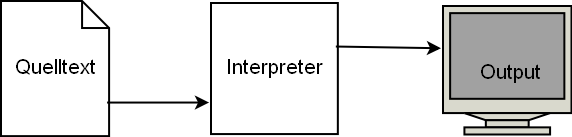
\includegraphics[scale=0.4]{graphics/interpreter.png}
	\caption{Interpreter}
	\label{fig:interpreter}
\end{figure}

Ein Compiler analysiert das Programm und �bersetzt es komplett, bevor das Programm ausgef�hrt wird. Der somit entstandene Code wird Objektcode genannt. Das Programm kann ohne weitere �bersetzung wiederholt ausgef�hrt werden.

\begin{figure}[ht]
	\centering
	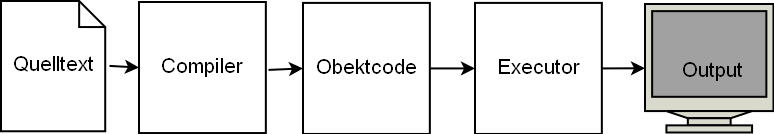
\includegraphics[scale=0.4]{graphics/compiler.png}
	\caption{Compiler}
	\label{fig:compiler}
\end{figure}

Python wird zu den interpretierten Programmiersprachen gez�hlt; Programme werden von einem Interpreter ausgef�hrt. Es gibt hierbei zwei Varianten: den Kommandozeilenmodus und den Skriptmodus. Im Kommandozeilenmodus werden Befehle Zeile f�r Zeile eingegeben, der Interpreter gibt das Ergebnis sofort retour\footnote{Im Laufe der Arbeit werden immer wieder Quelltexte eingearbeitet. Dabei gibt es zwei Formen. Die interaktive Session einer Interpreter Shell und den Skriptmodus. Die Interpreter Sessions sind erkennbar an der typischen Python Eingabeaufforderung (engl. "'prompt"'), die durch drei aufeinanderfolgende spitze Klammern ($>>>$) symbolisiert wird. Die Eingabe ist dabei immer fett ausgepr�gt, die Ausgabe des Interpreters normal.}:

\begin{lstlisting}[style=interpreter, label=python:first_example]
$ python
Python 2.4.4c1 (#1, Oct 13 2006, 12:10:43)
Type "help", "copyright", "credits" or "license" for more information. 
>>> print 10 * 2 
20
\end{lstlisting}

Im Skriptmodus wird das Programm in einem File gespeichert. Der Inhalt wird dann vom Interpreter ausgef�hrt.

Der Skriptmodus f�hrt zum Begriff Skriptsprache. Wie zu Beginn des Kapitels erw�hnt, wird Python den interpretierten Skriptsprachen zugeordnet.
Eine Skriptsprache ist eine \HLL\/, jedoch mit noch h�herer Abstraktion zur Maschine. \cite{python:scriptinglanguages} unterscheidet dabei Systemsprachen von Skriptsprachen wie folgt:
\begin{quote}
{\itshape "'Scripting languages are designed for different tasks than system programming languages, and this leads to fundamental differences in the languages. System programming languages were designed for building data structures and algorithms from scratch, starting from the most primitive computer elements such as words of memory. In contrast, scripting languages are designed for gluing: they assume the existence of a set of powerful components and are intended primarily for connecting components together. [...] Scripting languages are sometimes referred to as glue languages or system integration languages. [...] The growth of the Internet has also popularized scripting languages. The Internet is nothing more than a gluing tool."'}
\end{quote}

Skriptsprachen haben andere Aufgaben als "'Systemsprachen"'. Sie sind nicht darauf ausgelegt Datenstrukturen oder Algorithmen von Grund auf neu zu entwickeln, sondern als Bindeglied f�r vorhandene Applikationen zu dienen. Skriptsprachen bedienen sich also anderer Komponenten, um daraus eine eigene Applikation entstehen zu lassen.

Den immer wieder kritisierten Geschwindigkeitsunterschied zu kompilierten Sprachen versuchen Skriptsprachen wie Python zu verbessern. So wird der Quelltext nicht direkt interpretiert, sondern zuerst in den sogenannten "'Bytecode"' umgewandelt. Dieser wird wesentlich schneller interpretiert. Wirklich Geschwindigkeitskritisches  oder Rechenintensives wird in einer kompilierten Sprache geschrieben. Wie schon erw�hnt, wird bei Python C verwendet. Weiters relativiert immer schnellere und billigere Hardware die Kritik an der Performance.

Einige weitere Eigenschaften von Skriptsprachen sind in diesem Kapitel schon erw�hnt. Zur �bersicht sei eine Darstellung in kompakter Form aufgelistet:
\begin{itemize}
	\item noch "'h�here"' Implementierung als eine typische \HLL\
	\item interpretiert
	\item dynamische Typverwaltung
	\item optimal f�r schnelle Softwareentwicklung bzw. Prototyping \cite{python:linkweiler}
	\item hoher Re-Use Faktor
	\item leichter erlernbar als Systemsprachen
\end{itemize}

Weitere Beispiele f�r Skriptsprachen sind Perl\footnote{Perl: http://www.perl.com/} oder Tcl\footnote{Tcl: http://www.tcl.tk/}.		
